%%% LaTeX Template: Article/Thesis/etc. with colored headings and special fonts
%%%
%%% Source: http://www.howtotex.com/
%%% Feel free to distribute this template, but please keep to referal to http://www.howtotex.com/ here.
%%% February 2011
%%%
%%% Modified January 2016 by CDM

%%%  Preamble
\documentclass[11pt,letterpaper]{article}
\usepackage[margin=1.0in]{geometry}
\usepackage[T1]{fontenc}
\usepackage[bitstream-charter]{mathdesign}
\usepackage[latin1]{inputenc}					
\usepackage{amsmath}						
\usepackage{xcolor}
\usepackage{cite}
\usepackage{hyphenat}
\usepackage{graphicx}
\usepackage{float}
\usepackage{subfigure}
\usepackage{sectsty}
\usepackage[compact]{titlesec} 
\usepackage[tablegrid]{vhistory}
\usepackage{pbox}
\allsectionsfont{\color{accentcolor}\scshape\selectfont}

%%% Definitions
\definecolor{accentcolor}{rgb}{0.0,0.0,0.5} 
\newcommand{\teamname}{Team Friendship}
\newcommand{\productname}{Back Burner Brew}
\newcommand{\coursename}{CSE 4316: Senior Design I}
\newcommand{\semester}{Spring 2021}
\newcommand{\docname}{Architectural Design Specifications}
\newcommand{\department}{Department of Computer Science \& Engineering}
\newcommand{\university}{The University of Texas at Arlington}
\newcommand{\authors}{Luke Brown \\ Marcos Juarez Casillas \\ Ju Young Isa Jung \\ Sujan Dumaru \\ Sunghwa Cho \\ Matthew Francis Schultz}

%%% Headers and footers
\usepackage{fancyhdr}
	\pagestyle{fancy}						% Enabling the custom headers/footers
\usepackage{lastpage}	
	% Header (empty)
	\lhead{}
	\chead{}
	\rhead{}
	% Footer
	\lfoot{\footnotesize \teamname \ - \semester}
	\cfoot{}
	\rfoot{\footnotesize page \thepage\ of \pageref{LastPage}}	% "Page 1 of 2"
	\renewcommand{\headrulewidth}{0.0pt}
	\renewcommand{\footrulewidth}{0.4pt}

%%% Change the abstract environment
\usepackage[runin]{abstract}			% runin option for a run-in title
%\setlength\absleftindent{30pt}			% left margin
%\setlength\absrightindent{30pt}		% right margin
\abslabeldelim{\quad}	
\setlength{\abstitleskip}{-10pt}
\renewcommand{\abstractname}{}
\renewcommand{\abstracttextfont}{\color{accentcolor} \small \slshape}	% slanted text

%%% Start of the document
\begin{document}

%%% Cover sheet
{\centering \huge \color{accentcolor} \sc \textbf{\department \\ \university} \par}
\vspace{1 in}
{\centering \huge \color{accentcolor} \sc \textbf{\docname \\ \coursename \\ \semester} \par}
\vspace{0.5 in}
\begin{figure}[h!]
	\centering
   	
\includegraphics[width=0.50\textwidth]{images/title.PNG}
\end{figure}
\vspace{0.5 in}
{\centering \huge \color{accentcolor} \sc \textbf{\teamname \\ \productname} \par}
\vspace{0.5 in}
{\centering \large \sc \textbf{\authors} \par}
\newpage


%\vspace{1 in}
%\centerline{January 13th, 2012}
%\newpage

%%% Revision History
\begin{versionhistory}
  	\vhEntry{0.1}{10.01.2015}{GH}{document creation}
  	\vhEntry{0.2}{10.05.2015}{AT|GH}{complete draft}
  	\vhEntry{0.3}{10.12.2015}{AT|GH}{release candidate 1}
  	\vhEntry{1.0}{10.20.2015}{AT|GH|CB}{official release}
  	\vhEntry{1.1}{10.31.2015}{AL}{added design review requests}
\end{versionhistory}
\newpage

%%% Table of contents
\setcounter{tocdepth}{2}
\tableofcontents
\newpage

%%% List of figures and tables (optional)
\listoffigures
\listoftables
\newpage

%%% Document sections
\section{Introduction}
The "Back Burner Brew" is built with the sole purpose of brewing large batch of beer in the home environment. This product provides home brewers with a low-cost electric home brewing system that allow them to have precise control over the brewing process. The brewing process can be automated with the help of micro-controllers like the Raspberry Pi, ESP32 which is then hosted to a local website or an app interface.

ESP32 is a micro-controller that can receive data such as current temperature of the water or mash from the heat sensors located inside the kettles which can be converted to either analog or digital input. The heating coil can be controled using the input from the user as per their desired either to increase or to decrease the temperature. The electric pump can also be controlled by the user through micro-controllers to regulate the flow of the water in the kettles. The user will be able to communicate with the brewing system through a web interface.

The user should expect to input desired commands, controls, and specific
settings such as temperature and length of time through web interface.
The user can expect that whichever temperature they set for their desired
application, that the temperature will remain constant.

The intended audiences for this product would be home brewers or person interested in brewing beer only. Provided that the user manual would be present in the product, any person who wants to brew beer in his local environment can easily use this product. This product is made focusing on how effortless can the brewing process gets simply with the use of micro-controller.
\newpage
\section{System Overview}
This section should describe the overall structure of your software system. Think of it as the strategy for how you will build the system. An architectural "layer" is the top-level logical view, or an abstraction, of your design. Layers should be composed of related elements of similar capabilities, and should be highly independent of other layers, but should have very clearly defined interfaces and interactions with other layers. Each layer should be identified individually and should be unique as to its function and purpose within the system. This section should also contain the high-level block diagram of the layers, as shown in the example below, as well as detailed descriptions of the functions of each layer.

\begin{figure}[H]
	\centering
	\graphicspath{.\images}
	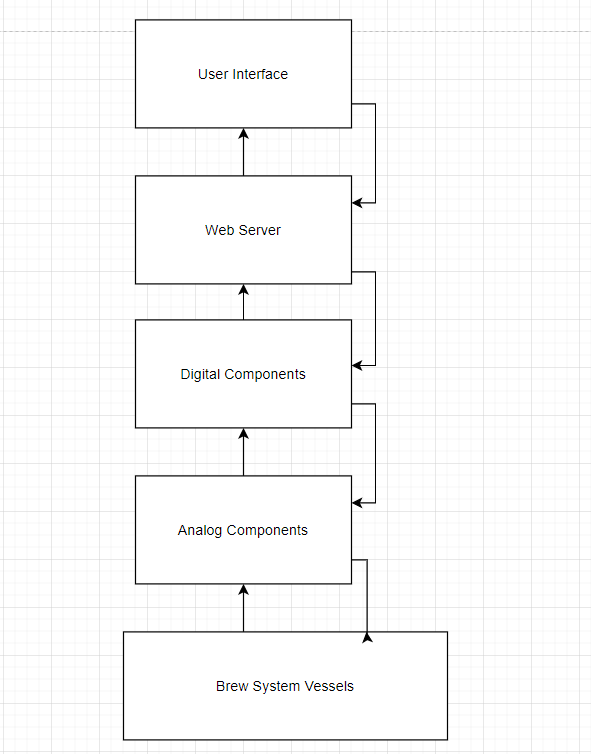
\includegraphics[scale=0.5]{images/simple_ads.PNG}
	\caption{Simple ADS}
\end{figure}
\subsection{Layer X Description}
Each layer should be described separately in detail. Descriptions should include the features, functions, critical interfaces and interactions of the layer. The description should clearly define the services that the layer provides. Also include any conventions that your team will use in describing the structure: naming conventions for layers, subsystems, modules, and data flows; interface specifications; how layers and subsystems are defined; etc. 

\subsection{Layer Y Description}
Each layer should be described separately in detail. Descriptions should include the features, functions, critical interfaces and interactions of the layer. The description should clearly define the services that the layer provides. Also include any conventions that your team will use in describing the structure: naming conventions for layers, subsystems, modules, and data flows; interface specifications; how layers and subsystems are defined; etc. 

\subsection{Layer Z Description}
Each layer should be described separately in detail. Descriptions should include the features, functions, critical interfaces and interactions of the layer. The description should clearly define the services that the layer provides. Also include any conventions that your team will use in describing the structure: naming conventions for layers, subsystems, modules, and data flows; interface specifications; how layers and subsystems are defined; etc. 
\newpage
\section{Subsystem Definitions \& Data Flow}
This section breaks down your layer abstraction to another level of detail. Here you grapically represent the logical subsytems that compose each layer and show the interactions/interfaces between those subsystems. A subsystem can be thought of as a programming unit that implements one of the major functions of the layer. It, therefore, has data elements that serve as source/sinks for other subsystems. The logical data elements that flow between subsystems need to be explicitly defined at this point, beginning with a data flow-like diagram based on the block diagram.

\begin{figure}[H]
	\centering
	\graphicspath{.\images}
	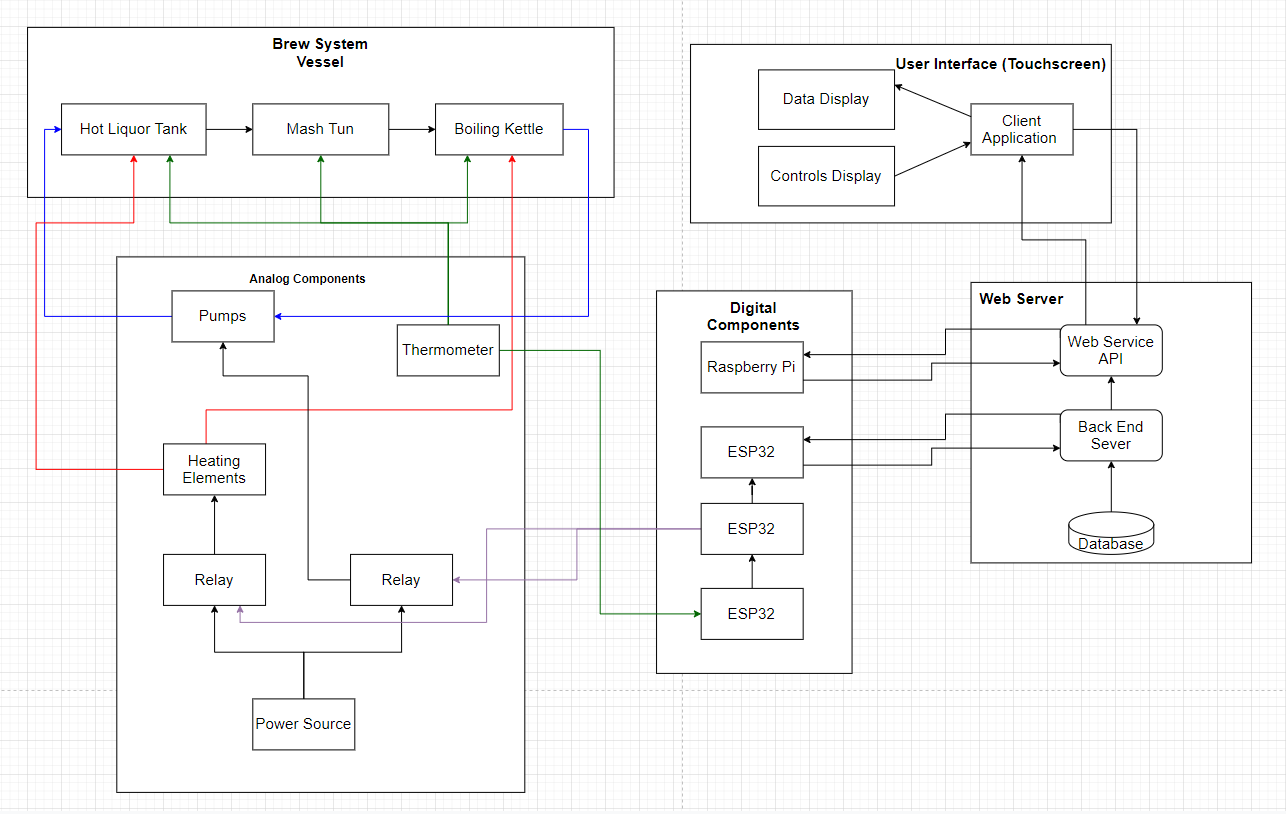
\includegraphics[scale=0.5]{images/ADS_system.PNG}
	\caption{Subsystem ADS}
\end{figure}
\newpage
\section{Brew System Vessel Layer Subsystems}
In this section, the layer is described in some detail in terms of its specific subsystems. Describe each of the layers and its subsystems in a separate chapter/major subsection of this document. The content of each subsystem description should be similar. Include in this section any special considerations and/or trade-offs considered for the approach you have chosen.

\subsection{Subsystem 1}
This section should be a general description of a particular subsystem for the given layer. For most subsystems, an extract of the architectural block diagram with data flows is useful. This should consist of the subsystem being described and those subsystems with which it communicates.

\begin{figure}[h!]
	\centering
 	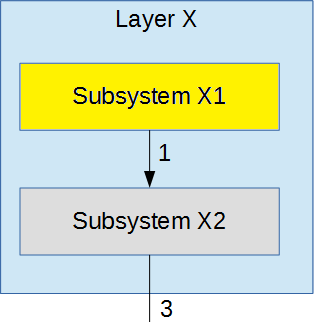
\includegraphics[width=0.60\textwidth]{images/subsystem}
 \caption{Example subsystem description diagram}
\end{figure}

\subsubsection{Assumptions}
Any assumptions made in the definition of the subsystem should be listed and described. Pay particular attention to assumptions concerning interfaces and interactions with other layers.

\subsubsection{Responsibilities}
Each of the responsibilities/features/functions/services of the subsystem as identified in the architectural summary must be expanded to more detailed responsibilities. These responsibilities form the basis for the identification of the finer-grained responsibilities of the layer's internal subsystems. Clearly describe what each subsystem does.

\subsubsection{Subsystem Interfaces}
Each of the inputs and outputs for the subsystem are defined here. Create a table with an entry for each labelled interface that connects to this subsystem. For each entry, describe any incoming and outgoing data elements will pass through this interface.

\begin {table}[H]
\caption {Subsystem interfaces} 
\begin{center}
    \begin{tabular}{ | p{1cm} | p{6cm} | p{3cm} | p{3cm} |}
    \hline
    ID & Description & Inputs & Outputs \\ \hline
    \#xx & Description of the interface/bus & \pbox{3cm}{input 1 \\ input 2} & \pbox{3cm}{output 1}  \\ \hline
    \#xx & Description of the interface/bus & \pbox{3cm}{N/A} & \pbox{3cm}{output 1}  \\ \hline
    \end{tabular}
\end{center}
\end{table}

\subsection{Subsystem 2}
Repeat for each subsystem

\subsection{Subsystem 3}
Repeat for each subsystem


\newpage
\section{Analog Components Layer Subsystems}
The Analog components layer contains 6 components. Five of the components will be actively interacting with each other. Being the pumps and heating elements will be controlled by the relays will be drawing power from the power supply. The thermometer will be interacting with the Digital component and Brew System Vessel Layers.

\begin{figure}[h!]
	\centering
	\graphicspath{.\images}
	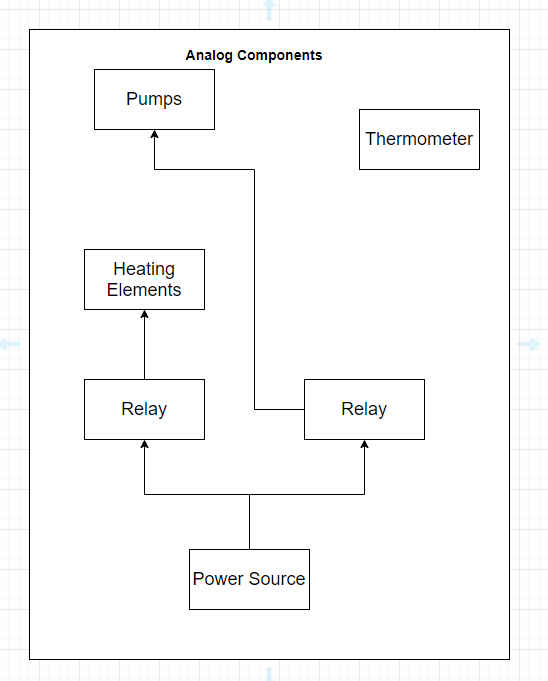
\includegraphics[scale=0.5]{images/analog_layer.PNG}
	\caption{Analog Components Layer}
\end{figure}

\subsection{Heating Elements Subsystem 1}
This subsystem is the temperature control subsystem used for managing temperature of the Hot Liquor tank and the Boiling Kettle. The Heating Elements will be managed by a relay that will be receiving control signals from a ESP32. 


\subsubsection{Assumptions}
We will be able to effectively manage the temperature of the Brewing system by increasing or decreasing temperature of heating elements. That is, logic on the digital components will be handling the optimal path to reach a certain temperature and the Relay will simply manage power to Heating Elements.  

\subsubsection{Responsibilities}
The subsystem will be responsible for temperature control of the brewing process.

\subsubsection{Subsystem Interfaces}

\begin {table}[H]
\caption {Subsystem interfaces} 
\begin{center}
    \begin{tabular}{ | p{4cm} | p{6cm} | p{5cm} | p{8cm} |}
    \hline
    Description & Inputs & Outputs \\ \hline
    Heating Elements & \pbox{5cm}{Power regulated by Relay} & \pbox{8cm}{Heat applied to Brew System}  \\ \hline
    Relay & \pbox{5cm}{Control information from ESP32} & \pbox{8cm}{Power to Heating Elements}  \\ \hline
    \end{tabular}
\end{center}
\end{table}


\subsection{Pump Control System Elements Subsystem 2}
This system will perform flow control from the Boiling Kettle to the Hot Liquor Tank. Like the Heating Elements, the Pumps will be controlled by a relay that is receiving control signals from an ESP32.    

\subsubsection{Assumptions}
The system will be designed to achieve a desired brew. You will only need this system to know when to turn on and off the pump from the Boiling Kettle to the Hot Liquor Tank.    

\subsubsection{Responsibilities}
The subsystem will be used for managing the pumping of liquid from the Boiling Kettle to the Hot Liquor Tank.

\subsubsection{Subsystem Interfaces}

\begin {table}[H]
\caption {Subsystem interfaces} 
\begin{center}
    \begin{tabular}{ | p{4cm} | p{6cm} | p{5cm} | p{8cm} |}
    \hline
    Description & Inputs & Outputs \\ \hline
    Heating Elements & \pbox{5cm}{Fluid from the Boiling Kettel \\ Power regulated by Relay} & \pbox{8cm}{Fluid to the Hot Liquor Tank}  \\ \hline
    Relay & \pbox{5cm}{Control information from ESP32} & \pbox{8cm}{Power moderation for Pumps}  \\ \hline
    \end{tabular}
\end{center}
\end{table}

\subsection{Power Relay Subsystem 3}
The power relay subsystem consist of the Relays and the Power Source. Relays will be used for managing power based on control signals from ESP32 to the Relays.     



\subsubsection{Assumptions}
The Relays will be connected to the Power Source and to the device it is controlling. The Relays will be able to operate on ESP32 inputs simply managing power to the devices.     

\subsubsection{Responsibilities}
This subsystem will be managing the power to devices that control elements of the Brew System Vessel.

\subsubsection{Subsystem Interfaces}

\begin {table}[H]
\caption {Subsystem interfaces} 
\begin{center}
    \begin{tabular}{ | p{5cm} | p{6cm} | p{5cm} | p{8cm} |}
    \hline
    Description & Inputs & Outputs \\ \hline
    Heating Elements & \pbox{5cm}{ESP32 control signals \\ Power from Power Source} & \pbox{5cm}{Power to device}  \\ \hline
    Relay & \pbox{5cm}{ESP32 control signals \\ Power from Power Source} & \pbox{5cm}{Power to device}  \\ \hline
    \end{tabular}
\end{center}
\end{table}


\subsection{Thermometer Subsystem 4}
This subsystem contains only one component, the Thermometer. It will be used for measuring the temperature of the Brew System and will relay that information to an ESP32.    



\subsubsection{Assumptions}
The Thermometer will have some other power supply. The ESP32 will take the temperature information and will know what to do when given the information.   

\subsubsection{Responsibilities}
This subsystem will be transporting temperature data from the Brew System to the necessary ESP32 were the information is required.  

\subsubsection{Subsystem Interfaces}

\begin {table}[H]
\caption {Subsystem interfaces} 
\begin{center}
    \begin{tabular}{ | p{5cm} | p{6cm} | p{5cm} | p{8cm} |}
    \hline
    Description & Inputs & Outputs \\ \hline
    Thermometer & \pbox{5cm}{Temperature measurements of Brew System Components} & \pbox{5cm}{Temperature data of Brew System}  \\ \hline
    
    \end{tabular}
\end{center}
\end{table}



\newpage
\section{Digital Components Layer Subsystems}
The digital components layer will consist of 4 devices. The first is a Raspberry
PI. This will act as the main computer of the system. It will the major hub for
the data both from the server: the UI, and the micro controllers. The other 3
components will all be ESP32 micro controllers, but they will each serve a
different purpose. An ESP32 will receive information from a thermometer sensor
and relay it to the heat control ESP32. Based on what the temperature is, the
heat control ESP32 will trigger the relay to activate or deactivate the heating
element. The final ESP32 will be used to trigger the relay to turn on the pump
based on what the message broker instructs it to do.   

\begin{figure}[h!]
	\centering
 	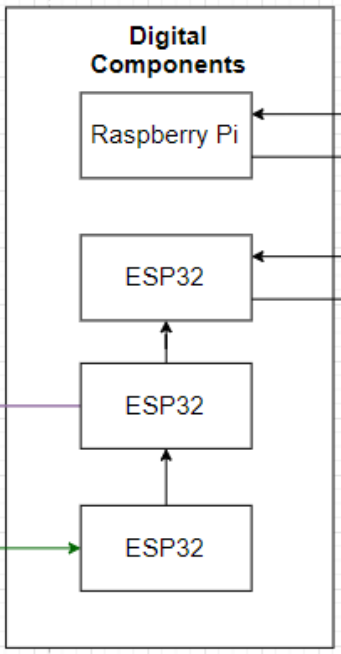
\includegraphics[width=0.30\textwidth]{images/digital_components.png}
  \caption{Digital Components Subsystem Description Diagram}
\end{figure}

\subsection{Raspberry PI Subsystem}
The Raspberry PI will host the web server and the MQTT client. The Raspberry PI will
receive information from the web server about what the user inputted via the UI.
It will then take that information and relay it to the micro controllers using
the MQTT protocol. The Raspberry PI will then receive sensor data from the
micro controllers through MQTT protocol and send the information in the web
server for storing. 

\subsubsection{Assumptions}
The Raspberry PI will have a power supply. It will remain safe from the elements. It
will be connected to the network. It will have unbroken communication with the
web server. It will communicate with the micro controllers through the MQTT protocol.

\subsubsection{Responsibilities}
It will receive data from the web server to determine how to operate the pump.
It will instruct the micro-controller to activate or deactivate based on the
information it receives. It will relay sensor information to the web server so
that it can be displayed.

\subsubsection{Subsystem Interfaces}
\begin {table}[H]
  \caption {Raspberry Pi Subsystem interfaces} 
  \begin{center}
    \begin{tabular}{ | p{5cm} | p{4cm} | p{4cm} |}
      \hline
      Description & Inputs & Outputs \\ \hline
      Web Service API & \pbox{4cm}{Information from UI input by user} & \pbox{4cm}{Sensor Data and status}  \\ \hline
      ESP32 & \pbox{4cm}{Sensor data from ESP32} & \pbox{4cm}{Messages instructing microcontrollers what to do}  \\ \hline
    \end{tabular}
  \end{center}
\end{table}

\subsection{Thermometer Sensor Subsytem}
This micro-controller will monitor data from the thermometer sensor. It will then
relay that information back to the message broker. 

\subsubsection{Assumptions}
The microcontroller will have a power supply. It will remain safe from the elements. It
will be connected to the network. It will be connected to the thermometer
sensor. It will operate through MQTT protocol.

\subsubsection{Responsibilities}
It will monitor the data from the thermometer sensor and relay that information
using the MQTT protocol. 

\subsubsection{Subsystem Interfaces}
\begin {table}[H]
  \caption {Thermometer Sensor Subsystem interfaces} 
  \begin{center}
    \begin{tabular}{ | p{5cm} | p{4cm} | p{4cm} |}
      \hline
      Description & Inputs & Outputs \\ \hline
      Thermometer Sensor & \pbox{4cm}{Data from thermometer sensor} & \pbox{4cm}{message to communicate sensor data}  \\ \hline
    \end{tabular}
  \end{center}
\end{table}

\subsection{Heat Control Subsystem}
The microcontroller will await messages from the message broker. The message
broker will receive information from the thermometer ESP32. If the temperature
is too low, the message broker will send a message to this microcontroller to
trigger the relay and allow power to flow to the heating element. If the
temperature gets too high on the heating element, the message broker will tell
this microcontroller to deactivate the heating element.

\subsubsection{Assumptions}
The microcontroller will have a power supply. It will remain safe from the elements. It
will be connected to the network. It will be connected to the relay that
controls power to the heating element. It will operate through MQTT protocol.

\subsubsection{Responsibilities}
It will activate or deactivate the relay that controls the power flow to the
heating element based on what the message broker instructs it to do. It will
send a status message back to the message broker. 

\subsubsection{Subsystem Interfaces}
\begin {table}[H]
  \caption {Heat Control Subsystem interfaces} 
  \begin{center}
    \begin{tabular}{ | p{5cm} | p{4cm} | p{4cm} |}
      \hline
      Description & Inputs & Outputs \\ \hline
      Heating Element Relay & \pbox{4cm}{message from RBP} & \pbox{4cm}{relay trigger and status message}  \\ \hline
    \end{tabular}
  \end{center}
\end{table}

\subsection{Pump Control Subsystem}
This microcontroller will await messages from the message broker. When the
message broker sends it the message to turn on the pump, the microcontroller
will trigger the relay to allow power to go to the pump. When the message broker
sends the message to turn off the pump, the microcontroller will cease sending
power to the relay, causing it to close, and power will not be supplied to the
pump.

\subsubsection{Assumptions}
The microcontroller will have a power supply. It will remain safe from the elements. It
will be connected to the network. It will be connected to the pump relay. It will operate through MQTT protocol.

\subsubsection{Responsibilities}
It will trigger the relay that will supply power to the pump based on the
message it receives from the message broker. It will then return a status
message to the message broker.

\subsubsection{Subsystem Interfaces}

\begin {table}[H]
\caption {Pump Control Subsystem interfaces} 
\begin{center}
    \begin{tabular}{ | p{6cm} | p{3cm} | p{3cm} |}
    \hline
    Description & Inputs & Outputs \\ \hline
    Pump Relay & \pbox{3cm}{message from RBP} & \pbox{3cm}{relay trigger and status message}  \\ \hline
    \end{tabular}
\end{center}
\end{table}

\newpage
\section{Web Server Layer Subsystems}
The Web Server Layer will receive and store data gained from Raspberry Pi and provide web service API to front-end applications. Online or local databases will be used such as Google Firebase, Amazon RDS, Mysql, etc. Web service API will provide information to the devices when they call in order to meet the criteria set by the brewer. The web server should be able to get a recipe from a user and control heating elements and the pumps based on conditions of water temperature and the amount of time that a user set for brewing.

\subsection{Web Service API}
API is a software interface that allows two applications to interact with each other without any user involvement. Web service API will provide information extracted from the database to the user interface layer when certain APIs are called.

\begin{figure}[h!]
	\centering
 	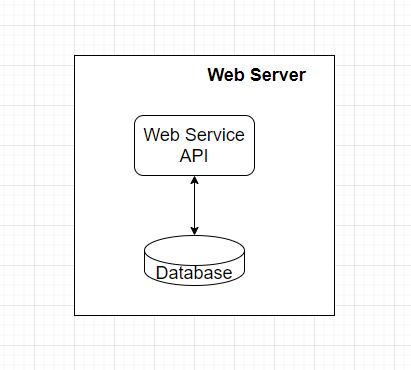
\includegraphics[width=0.60\textwidth]{images/web_layer.PNG}
 \caption{Example subsystem description diagram}
\end{figure}

\subsubsection{Assumptions}

\begin {itemize}
\item 
The Web service API supports HTTP/HTTPS protocol. is used for transferring data.
\item 
Web service supports XML and JSON.
\item 
Web service is RESTful (GET, POST, PUT and DELETE).
\end {itemize}


\subsubsection{Responsibilities}
Web Service API should establish stable connections with database and HTTP protocols to transfer data without data leak. Each corresponding APIs will extract accurate information from the database and provide it to other devices to help them to make the correct decision. 

\subsubsection{Subsystem Interfaces}

\begin {table}[H]
\caption {Subsystem interfaces} 
\begin{center}
    \begin{tabular}{| p{6cm} | p{3cm} | p{3cm} |}
    \hline
    Description & Inputs & Outputs \\ \hline
    API called from other devices & \pbox{3cm}{user input} & \pbox{3cm}{Data}  \\ \hline
    \end{tabular}
\end{center}
\end{table}

\subsection{Database}
A database is a data structure that stores organized information with multiple tables, which may each include several different fields. The brewing database may include tables for water temperature, recipe, etc. Each of these tables would have different fields that are relevant to the information stored in the table.

\begin{figure}[h!]
	\centering
 	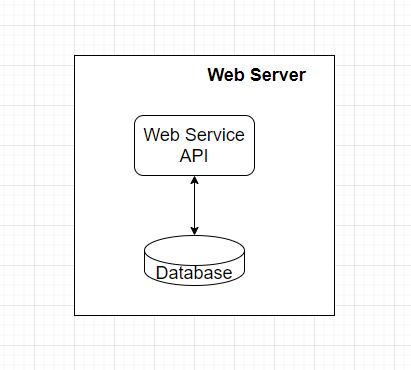
\includegraphics[width=0.60\textwidth]{images/web_layer.PNG}
 \caption{Example subsystem description diagram}
\end{figure}

\subsubsection{Assumptions}

\begin {itemize}
\item Database should establish a stable connection with Web service API.
\end {itemize}


\subsubsection{Responsibilities}
The database should be available at any time and have enough capacity to store data. 

\subsubsection{Subsystem Interfaces}

\begin {table}[H]
\caption {Subsystem interfaces} 
\begin{center}
    \begin{tabular}{| p{6cm} | p{3cm} | p{3cm} |}
    \hline
    Description & Inputs & Outputs \\ \hline
    Receive requests from API & \pbox{3cm}{query from API} & \pbox{3cm}{Data}  \\ \hline
    \end{tabular}
\end{center}
\end{table}



\newpage
\section{User Interface Layer Subsystems}
The touchscreen device will retrieve application data from the web server to display information from the current brew.  The display will also offer a Graphical User interface where the user can input commands to modify the current brew. The client application running on this device will then interpret the data, and either display it on the Data Display or send it back to the server as commands accordingly.

\subsection{Data Display}
The data display will display real-time information relevant to the current brew. The data display will retrieve this data from the web server.

\begin{figure}[h!]
	\centering
 	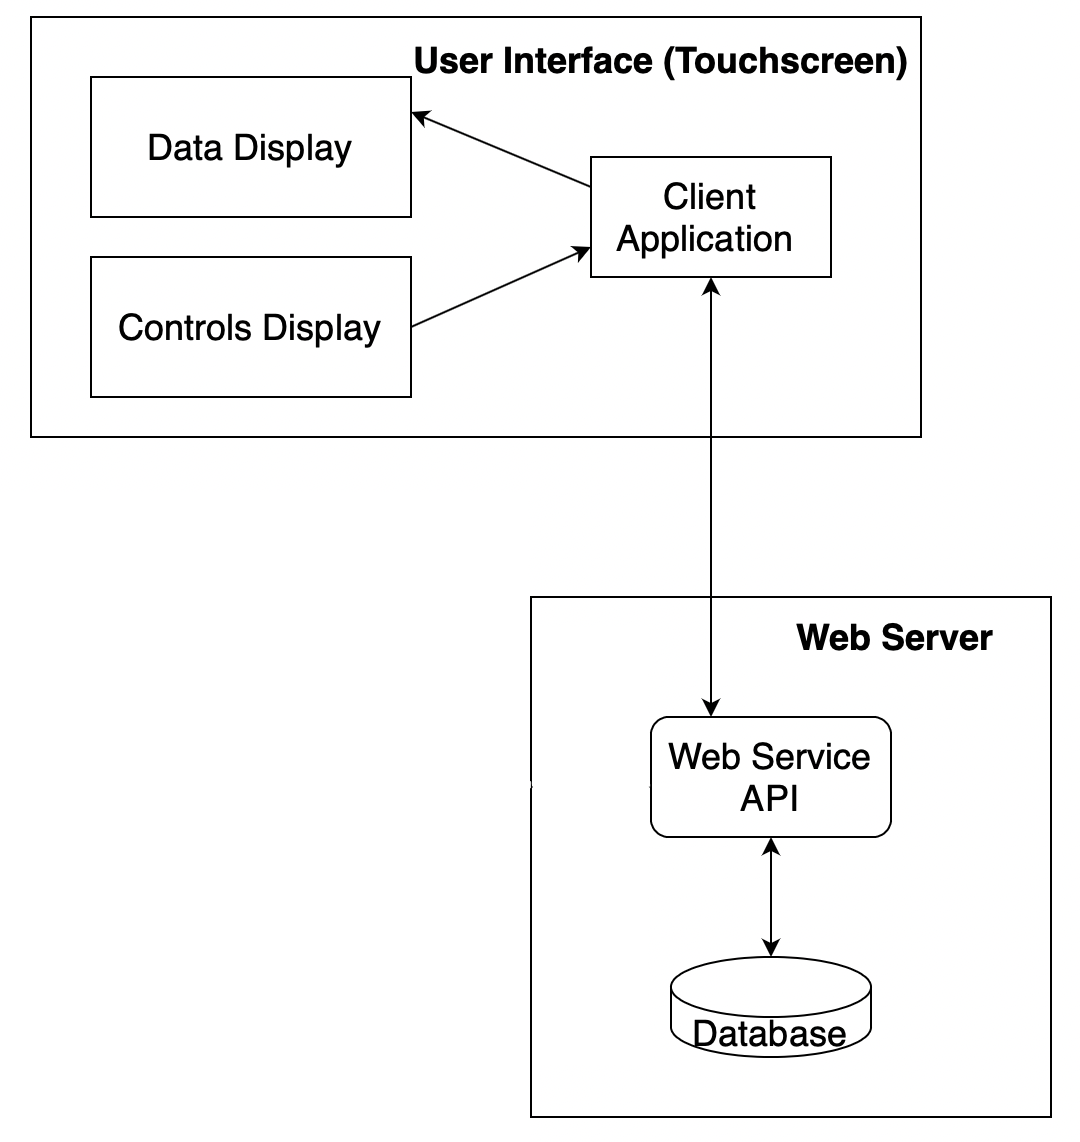
\includegraphics[width=0.60\textwidth]{images/UI_subsystem}
 \caption{User Interface subsystem diagram}
\end{figure}

\subsubsection{Assumptions}
\begin {itemize}
\item The device will receive the data and interpret it correctly on the touchscreen.
\item The data received from the server will be accurate and up-to-date.
\item The device will have a stable connection to the server throughout the brew.
\end {itemize}


\subsubsection{Responsibilities}
The device will receive accurate and relevant information from the server and display it on the touchscreen for the user to make decisions on the current brew. This information will include current set temperature, length of time the temperature has been set, how much longer brew will stay at current temperature, and any other information that may be relevant.

\subsubsection{Subsystem Interfaces}

\begin {table}[H]
\caption {Subsystem interfaces} 
\begin{center}
    \begin{tabular}{ | p{6cm} | p{3cm} | p{3cm} |}
    \hline
    Description & Inputs & Outputs \\ \hline
    Data Display & \pbox{3cm}{Data from \\ server} & \pbox{3cm}{Brew information}  \\ \hline
    \end{tabular}
\end{center}
\end{table}

\subsection{Controls Display}
The controls display on the touchscreen will allow the user to interact with and send commands to the server, which will relay the data to the brewing system.

\begin{figure}[h!]
	\centering
 	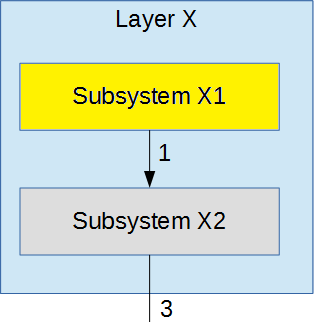
\includegraphics[width=0.60\textwidth]{images/subsystem}
 \caption{Example subsystem description diagram}
\end{figure}

\subsubsection{Assumptions}
\begin {itemize}
\item The client application will read user commands correctly and send them following the established protocol.
\item The device will be quick in sending commands to the server.
\item The device will have a stable connection to the server throughout the brew.
\end {itemize}


\subsubsection{Responsibilities}
The touchscreen will allow the user to enter commands such as set, increase, or decrease temperature and/or the length of time temperature is set. The interface will be intuitive and easy to use. The client application will then take the commands, and send them to the server following the set communcation protocol. Commands sent will update the information on the data display if applicable.

\subsubsection{Subsystem Interfaces}

\begin {table}[H]
\caption {Subsystem interfaces} 
\begin{center}
    \begin{tabular}{| p{6cm} | p{3cm} | p{3cm} |}
    \hline
    Description & Inputs & Outputs \\ \hline
    Controls Display & \pbox{3cm}{User input} & \pbox{3cm}{Data to \\ server}  \\ \hline
    \end{tabular}
\end{center}
\end{table}



\newpage

%%% References
%\bibliographystyle{plain}
%\bibliographystyle{reference/IEEEtran_custom}
%\bibliography{reference/refs}{}

\end{document}